\chapter{Ottimizzazione parametrica e valutazione delle performance}

L'obiettivo dell'ambiente di simulazione è quello di valutare le performance dell'algoritmo integrato per stabilire la migliore configurazione dei parametri in un dato contesto applicativo.
Data l'eterogeneità delle missioni, infatti, non è possibile stabilire una configurazione di parametri che sia ottimale per tutti gli scenari.

Come abbiamo già più volte sottolineato nei capitoli precedenti, l'obiettivo di uno sciame è quello di identificare, entro il tempo di autonomia, i target presenti nell'area di esplorazione.
Una valutazione delle performance, di conseguenza, può essere eseguita in considerazione del tempo impiegato per il rilevamento (o per l'esecuzione, se la missione lo richiede) di almeno il $95\%$ dei target (\textit{discovering time}).
Una migliore configurazione dei parametri in ingresso, in relazione alla strategia di coordinamento adottata, comporterà un \textit{discovering time} inferiore.

Un altro parametro per la valutazione delle performance è rappresentato dal numero di collisioni, che risulta importante per due ragioni fondamentali:
\begin{enumerate}
    \item \textit{Costi:} in un contesto reale, la perdita di un drone può avere un impatto economico piò o meno rilevante a seconda del tipo di UAV;
    \item \textit{Rischi:} la collisioni di un drone può avere ripercussioni anche sull'incolumità di persone o cose.
\end{enumerate}

Al fine di ottenere un risultato significativo da un punto di vista statistico, la valutazione delle performance di un insieme di parametri viene  valutata come media su più esecuzioni indipendenti del simulatore.

\section{Ottimizzazione basata su \\\textit{Differential Evolution}}

L’algoritmo \textit{Differential Evolution} è uno strumento software in grado di trovare la configurazione ottimale dei parametri per un problema caratterizzato da una specifica complessità. 
Risulta importante sottolineare che l’algoritmo \textit{Differential Evolution} non garantisce la soluzione ottima del problema, ma una soluzione ottimale, ovvero una soluzione “vicina” a quella ottima. 

Nel caso in oggetto, lo strumento \textit{Differential Evolution} è utilizzato per configurare i parametri relativi al coordinamento previsto dall’algoritmo integrato nel simulatore. 
L’obiettivo principale del simulatore, infatti, è quello di valutare l’impatto dei meccanismi di coordinamento di uno sciame di UAV sui diversi scenari applicativi. 

L’algoritmo \textit{DE} ricerca il valore ottimale per ciascun parametro di configurazione all’interno di un intervallo definito a priori. 
Gli estremi di tale intervallo devono essere scelti in modo accurato in relazione alle caratteristiche del contesto applicativo e alle specifiche reali dei droni e dei sensori di rilevamento.

\subsection{Funzionamento dell'algoritmo \textit{Differential Evolution}}

Il Differential Evolution è un algoritmo evolutivo capace di gestire correttamente funzioni non differenziabili e non lineari. 
La ricerca del valore ottimo inizia con una popolazione generata in modo casuale, dove i valori assunti da ciascun elemento sono vincolati ad intervalli scelti a priori. 
Ad ogni iterazione, viene calcolato il risultato di una funzione obiettivo, detta \textit{fitness function}, sui vettori di parametri della generazione corrente.
L'obiettivo è quello di minimizzare il risultato di questa funzione operando con i meccanismi di evoluzione differenziale.

Come molti algoritmi che rientrano in questa categoria, opera con tre operazioni fondamentali: mutazione, crossover, selezione. 
Lo spazio delle soluzioni viene esplorato attraverso dei vettori di parametri generati per differenza; questo comportamento si individua nell’operazione di mutazione. Questa rappresenta la maggior differenza con gli algoritmi genetici, che utilizzano l’operazione di crossover (rimescolamento di geni) come primo meccanismo di ricerca. 

Il Differential Evolution utilizza delle differenze pesate fra i vettori delle soluzioni al fine di perturbare la popolazione e non richiede, inoltre, la codifica binaria dei membri della popolazione.

\begin{figure}[H] 
    \captionsetup{justification=centering, margin=2cm, font=footnotesize}
    \begin{center}
    \makebox[\textwidth]{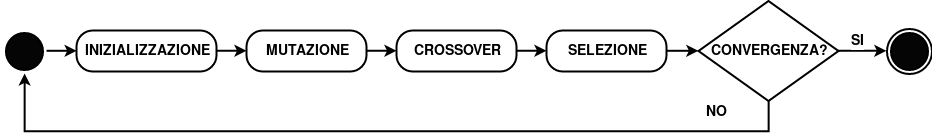
\includegraphics[width=0.6\paperwidth]{img/de_steps.png}}
    \end{center}
    \caption{Algoritmo Differential Evolution step-by-step.}
    \label{de_steps}
\end{figure}

Di seguito, si riporta lo pseudocodice del \textit{Differential Evolution}.
Nei paragrafi successivi, invece, verranno descritte nel dettaglio le tre operazioni fondamentali sopra introdotte.

\begin{figure}[H]
    \centering
    \begin{minipage}{\linewidth}
    \begin{algorithm}[H]
    \SetAlgoLined
        \Begin {
            generate randomly an initial population of solutions \;
            compute the fitness function of the initial population \;
            \While {stop condition !satisfied}{
                \For {each parent}{
                    select three solutions at random \;
                    create one offspring using the DE operators \;
                }
                \For {each member of the next generation}{
                    \If {offspring(x) is more fit than parent(x)}{
                        parent(x) is replaced \;
                    }
                }
            }
        }
    \end{algorithm}
    \end{minipage}
    \caption{Pseudocodice Differential Evolution.}
\end{figure}

\subsubsection{Mutazione}

Il meccanismo di mutazione è utilizzato per produrre una popolazione di $NP$ vettori, dove $NP$ rappresenta il numero di individui nella popolazione.
In particolare, questa operazione genera un nuovo vettore mutante, aggiungendo una frazione della differenza tra due vettori, selezionati casualmente, ad un terzo.

L'implementazione elementare di questa operazione è descritta dall'espressione di seguito riportata:
\begin{equation*}
    v_{i} = x_{r_{0}} \; + \; F(x_{r_{1}} - x_{r_{2}})
\end{equation*}
Dove:
\begin{itemize}
    \item $v_{i}$ è il nuovo vettore mutante;
    \item I termini $x_{r_i}$, con $i = 0,1,2$, rappresentano i tre vettori selezionati casualmente tra quelli disponibili;
    \item La funzione $F \in (0,1+)$ regola il tasso di evoluzione della popolazione.
\end{itemize}

\subsubsection{Crossover}

Questa operazione produce i vettori da testare a partire dai vettori di parametri.
In particolare, viene incrociato ogni vettore della popolazione attuale con un vettore mutante prodotto dall'operazione precedente.

L'espressione per descrivere la fase di crossover è la seguente:
\begin{equation*}
    u_{i} = \begin{cases}
        v_{i,j} \; , \text{se } rand_{j}(0,1) \leq Cr \\
        u_{i,j} \; , \text{altrimenti} 
    \end{cases}
\end{equation*}

In altre parole, il nuovo individuo viene generato scegliendo tra il vettore mutante e quello corrente, con una probabilità $Cr$, detta \textit{probabilità di crossover}.
Tale probabilità è un parametro definito dall'utente.

\subsubsection{Selezione}

Se il vettore della soluzione in uso, $u_{i}$, ottiene un valore della funzione obiettivo minore o uguale rispetto alla soluzione candidata migliore, questa viene sostituita dal vettore $u_{i}$ nella generazione successiva.
\begin{equation*}
    x_{i,g+1} = \begin{cases}
        u_{i,g} \; , \text{se } f(u_{i,g}) \leq f(x_{i,g}) \\
        x_{i,g} \; , \text{altrimenti} 
    \end{cases}
\end{equation*}

\subsection{Implementazione software \textit{Differential Evolution}}

Al fine di ottimizzare i parametri di simulazione, è stato implementato un modulo software di evoluzione differenziale, chiamato \textit{Differential\_evolution\_bridge}.
Attraverso tale modulo, è possibile calcolare la funzione obiettivo tramite l'esecuzione di una simulazione con il vettore di parametri passato in input alla funzione.

La \textit{fitness function} è calcolata come segue:
\begin{equation*}
    fitness(x) = \#ticks[simulation(x)]
\end{equation*}
Dove:
\begin{itemize}
    \item $x$ rappresenta l'individuo della generazione attuale, ovvero il vettore di parametri dato in input alla simulazione;
    \item $\#ticks$ rappresenta il numero di iterazioni necessarie al rilevamento del $95\%$ di target;
    \item $simulation(x)$ indica l'esecuzione di una sessione simulativa con i parametri di $x$.
\end{itemize}

Differential evolution bridge utilizza, come implementazione software dell’evoluzione differenziale, la procedura presente nella libreria Python Scipy.Optimize, denominata \textit{differential\_evolution}.
Il modello algoritmico seguito è quello offerto da Kenneth Price e Rainer Storn in \cite{storn1997differential}, implementato secondo la libreria Scipy \cite{jones2014scipy}.